\chapter{Literature Review}
\label{ch:LR}
\section{Taxonomy for Intrusion Detection Systems}

\paragraph{}
In \cite{ids_taxonomy}, an attempt has been made to standardize a terminology for IDSs. Many different types of common in use IDSs are introduced in the paper, along with some upcoming possibilities.

\paragraph{}
Broadly, IDSs have been classified on the basis of 5 different features (figure 2.1).
\begin{figure}[h]
    \hfill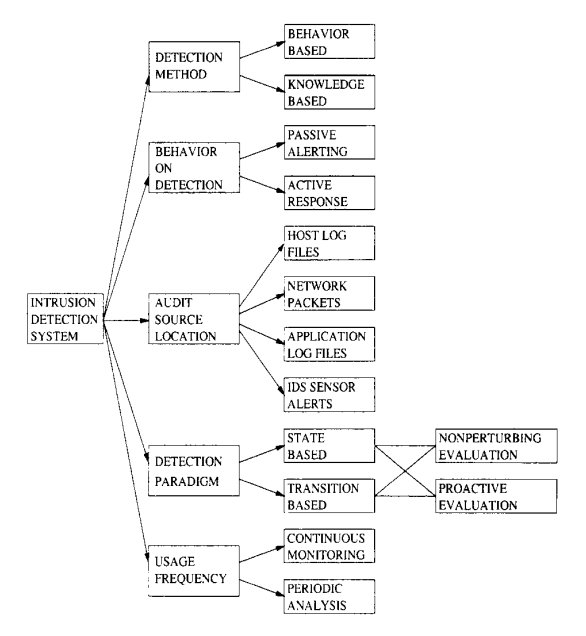
\includegraphics[width=0.8\textwidth]{Chapter2/types_of_ids}\hspace*{\fill}
    \caption{Types of IDS as mentioned in \cite{ids_taxonomy}}
    \label{}
\end{figure}
\begin{enumerate}
    \item On the basis of detection method:
        \begin{itemize}
            \item Behavior based
            \item Knwoledge based
        \end{itemize}
    \item On the basis of behavior on detection:
        \begin{itemize}
            \item Passive filtering
            \item Active filtering
        \end{itemize}
    \item On the basis of audit source location:
        \begin{itemize}
            \item Host log files
            \item Network packets
            \item Application log files
            \item IDS sensor alerts
        \end{itemize}
    \item On the basis of detection paradigm:
        \begin{itemize}
            \item State based
            \item Transition based
        \end{itemize}
    \item On the basis of usage frequency:
        \begin{itemize}
            \item Continuous monitoring
            \item Periodic analysis
        \end{itemize}
\end{enumerate}
